%%%%%%%%%%%%%%%%%%%%%%%%%%%%%%%%%
% Background and Literature Review %
%%%%%%%%%%%%%%%%%%%%%%%%%%%%%%%%%

\setlength{\arrayrulewidth}{0.5pt}
\renewcommand{\arraystretch}{1.3}
\section{Background and Literature Review}

This chapter establishes the conceptual and contextual foundations of the study. It presents the Tunisian banking sector and its regulatory environment, introduces the concept of data maturity, reviews existing data maturity frameworks, and identifies the research gaps the project addresses.

\subsection{Background}

The project's setting, the Tunisian banking sector and its regulatory environment, creates the need for a shared way of measuring and steering data maturity.

\subsubsection{The Tunisian Banking Sector}

The Tunisian banking sector is central to the national economy and faces growing regulatory attention regarding data management. Banks operate a large volume of transactional and customer data, yet the diagnostic conducted for this project found formal governance, automated quality control, and centralized architecture present in only a minority of respondents. This combination of data-intensive activity and uneven data management practices is the practical backdrop of the study.

\subsubsection{The Regulatory Environment}

Two regulatory references frame the expectations placed on banks. The Banque Centrale de Tunisie issued Circulaire N\textdegree{}2025-08\footnote{Banque Centrale de Tunisie, Circulaire N\textdegree{}2025-08 concerning data governance obligations, published 16~May 2025. Available at \url{https://www.bct.gov.tn}.}~\cite{bct2025}, which establishes structured expectations for data governance, ownership, and control within licensed institutions. In parallel, the international standard BCBS 239\footnote{Basel Committee on Banking Supervision, \emph{Principles for Effective Risk Data Aggregation and Risk Reporting} (BCBS~239), Bank for International Settlements, 2013. Available at \url{https://www.bis.org/publ/bcbs239.htm}.}~\cite{bcbs239}, issued by the Basel Committee on Banking Supervision, defines principles for effective risk data aggregation and reporting, emphasizing data accuracy, completeness, timeliness, and traceability. Together they converge on a single expectation: banks must demonstrate, in an auditable manner, that their data is governed, controlled, and traceable.

\textbf{BCT Circulaire N\textdegree{}2025-08.} The circular applies to all institutions licensed by the Banque Centrale de Tunisie; its data-governance obligations are set out in Article~6. For this study, four families of obligations were identified and mapped onto the assessment indicators; this mapping is the author's own reading of the text and remains pending validation by a compliance or legal authority. First, a data strategy must be formally approved by executive management, dated, and made accessible to the relevant stakeholders, so that an informal or verbal strategy does not satisfy the requirement. Second, data owners must be named individuals with documented accountability for each critical business domain, such as credit, risk, compliance, finance, and operations, supported by an accountability matrix that is communicated across the organization. Third, data validation rules must be automated rather than manual, documented with an owner and a last review date, and actively applied to incoming data flows in production. Fourth, the institution must maintain a formal, article-by-article mapping of its compliance obligations together with a pre-assembled evidence package, keeping it audit-ready and able to produce the supporting documents, system logs, and named responsible owners within a short delay. The circular also requires role-based access control with logged and periodically reviewed access grants, and the automated production of regulatory reports with a complete validation trail from source data to submitted output. These obligations are not skippable: they correspond to the thirteen indicators flagged as regulatory and treated as mandatory throughout the tool. Appendix~B maps each of these thirteen indicators to the obligation it operationalizes.

\textbf{BCBS 239.} BCBS 239 complements the national circular as an internationally recognized standard for risk data aggregation and reporting; issued by the Basel Committee, it formally binds globally systemic banks rather than Tunisian commercial banks, for which it nonetheless remains the recognized best-practice benchmark for risk data. The BCT circular's traceability and control expectations mirror it, so aligning with BCBS 239 both supports the national rule and future-proofs the bank. Its principles expect critical risk data to be accurate and reliable, complete across the relevant risk exposures, timely enough to support risk management decisions, and, above all, traceable. The traceability principle is the most operationally demanding: every critical risk data element used in a regulatory report must have documented lineage from source to report, auditable and kept current. Lineage recorded only in static office documents is treated as insufficient, because it cannot be verified or maintained at the scale of a bank's risk reporting. This standard therefore reinforces two maturity dimensions in particular, data quality and the lineage and traceability sub-dimension, and its expectations are embedded in the corresponding regulatory indicators rather than assessed separately.

\textbf{Convergence.} The two references are complementary rather than redundant. The BCT circular is prescriptive about governance structures, ownership, and audit readiness within the Tunisian jurisdiction, while BCBS 239 sets out principles for the technical quality and traceability of risk data. A bank satisfying only one would still carry material exposure: strong governance without traceable lineage leaves risk reports unverifiable, and traceable lineage without approved ownership leaves accountability undefined. The assessment framework designed in this work deliberately spans both, so that a single evaluation produces evidence relevant to both the national inspection and the international standard.

\subsubsection{The Concept of Data Maturity}

Data maturity refers to the degree to which an organization manages, governs, and exploits its data as a strategic asset. A maturity model expresses this degree along a progression of levels, typically ranging from ad hoc and reactive practices at the lowest level to optimized and systematically improved practices at the highest \cite{cmmi}. Maturity models serve two purposes: they provide a diagnostic snapshot of the current state, and they define a path of improvement toward a target state \cite{gartner}. In the data domain, maturity is commonly assessed across dimensions such as governance, quality, architecture, analytics, and organizational culture, each evaluated through a set of indicators \cite{dama2017}. One such indicator is D1.1-01, ``Is there a formally approved and dated data strategy document?'', a non-skippable regulatory indicator scored on a 1--5 scale against a rubric. In that rubric, level~1 means no strategy document exists, and level~3 means a strategy document has been formally approved by executive management, dated, and shared.

The value of a maturity model rests on three properties that distinguish it from a simple checklist. The first is graduation: rather than recording a binary presence or absence, the model places each practice on an ordered scale, so a practice existing informally is scored below the same practice documented, repeatable, and continuously improved. The second is evidence: a mature practice can be demonstrated, not merely asserted, which is why credible models tie their higher levels to documentary proof rather than intention. The third is actionability: because the levels are ordered, the distance between the current and a chosen target state defines a concrete improvement path, and the lowest scoring dimensions naturally surface as priorities. These three properties are precisely what a diagnostic instrument for banks must preserve, and they directly shape the scoring methodology adopted later in this work.

For a bank in particular, data maturity is not an abstract quality objective but a precondition for regulatory survival. A bank that cannot demonstrate governed, controlled, and traceable data cannot satisfy a supervisory inspection, cannot reliably aggregate risk data across its systems, and cannot trust the figures it submits in regulatory reports. Low data maturity therefore translates directly into regulatory exposure, remediation cost, and reputational risk. The study therefore treats maturity not as a purely managerial construct but as a measurable state with an auditable score, and weaves the regulatory expectations reviewed below into the maturity dimensions rather than treating them as a separate compliance exercise.

\subsection{Existing Related Studies}

This section reviews the existing data maturity frameworks that inform the design.

\subsubsection{Framework Selection Process}

The design of the hybrid framework began with a systematic screening of fifteen candidate data maturity and data management frameworks. The candidates spanned the five frameworks eventually retained as well as architecture, control, and quality standards such as TOGAF \cite{togaf}, COBIT 2019 \cite{cobit2019}, and ISO 8000 \cite{iso8000}. Each candidate was screened against five selection criteria: international credibility, banking relevance, scoring logic, complementarity with other candidate frameworks, and alignment with the BCT and BCBS 239 expectations. Each criterion was scored on a three point scale, where one denotes weak coverage, two moderate, and three strong, giving a maximum selection score of fifteen. Five frameworks were selected and ten were rejected. The full screening matrix is presented in Table~\ref{tab:framework-screening}.

The five criteria were chosen so that a framework scoring well on all of them would be usable, defensible, and complete for the banking context, and so that no single criterion could by itself justify selection. International credibility guards against citing proprietary or unpublished models that cannot be defended in academic work. Banking relevance rewards frameworks conceived for or widely adopted by financial institutions rather than generic enterprise IT. Scoring logic captures whether the framework provides an operational way to turn observations into a graded result, the property most descriptive frameworks lack. Complementarity is deliberately relational: it rewards a framework for filling a gap the other candidates leave open, which makes a hybrid combination coherent rather than a collection of overlapping models. Alignment with the BCT and BCBS 239 expectations ensures the regulatory obligations reviewed above are natively covered rather than bolted on afterward. Selection was not a pure score threshold: the five highest-scoring frameworks that are open and academically referenceable were selected, and proprietary or vendor-locked models were excluded even when their score was competitive. The McKinsey Data Model, for instance, scored 11 out of 15 but was rejected as proprietary and unpublished, and therefore not academically referenceable. The rationale for each decision is recorded in the decision column of Table~\ref{tab:framework-screening}.

The rejections were driven less by weak credibility than by two recurring failures that shape the hybrid design. The first is vendor or platform lock-in, which prevents an institution from applying the framework independently and blocks cross-institutional benchmarking. The second is narrow scope: a framework covers only one of the five required dimensions and so cannot support a full assessment. Throughout this work these five dimensions are labelled D1--D5: Governance (D1), Data Quality (D2), Architecture and Access (D3), Analytics and Tools (D4), and Skills and Culture (D5). Open publication and academic referenceability therefore acted as hard constraints rather than one score among many.

\begin{center}
{\footnotesize
\setlength{\tabcolsep}{4pt}
\begin{longtable}{|p{2.6cm}|c|c|c|c|c|c|p{5.8cm}|}
\caption{Framework screening matrix (15 candidates, 5 criteria)}\label{tab:framework-screening}\\

\hline
\textbf{Framework} & \textbf{IC} & \textbf{BR} & \textbf{SL} & \textbf{CP} & \textbf{BF} & \textbf{/15} & \textbf{Decision rationale} \\
\hline
\endfirsthead
\multicolumn{8}{c}{\footnotesize (Table~\ref{tab:framework-screening} continued)} \\[2pt]
\hline
\textbf{Framework} & \textbf{IC} & \textbf{BR} & \textbf{SL} & \textbf{CP} & \textbf{BF} & \textbf{/15} & \textbf{Decision rationale} \\
\hline
\endhead
\hline
\multicolumn{8}{r}{\footnotesize (continued on next page)} \\
\endfoot
\hline
\multicolumn{8}{|p{13cm}|}{\footnotesize \textbf{Criteria:} IC = International Credibility; BR = Banking Relevance; SL = Scoring Logic; CP = Complementarity; BF = BCT/BCBS Fit. Scale: 1 = Weak, 2 = Moderate, 3 = Strong.} \\
\hline
\endlastfoot
%% Selected frameworks
\multicolumn{8}{|l|}{\textbf{Selected frameworks (5)}} \\
\hline
DAMA-DMBOK      & 3 & 2 & 1 & 3 & 2 & \textbf{11} &
  \textit{Selected.} Structural backbone: 11 domains, taxonomy for the 5 dimensions. \\
\hline
DCAM            & 3 & 3 & 2 & 3 & 3 & \textbf{14} &
  \textit{Selected.} Regulatory anchor: only framework built for financial institutions. \\
\hline
CMMI-DMM        & 3 & 2 & 3 & 3 & 2 & \textbf{13} &
  \textit{Selected.} Maturity scale: 5 levels, evidence-based scoring logic. \\
\hline
TDWI Analytics  & 3 & 2 & 3 & 3 & 2 & \textbf{13} &
  \textit{Selected.} Evaluation engine: questionnaire structure, per-indicator rubrics. \\
\hline
Gartner D\&A Maturity & 3 & 2 & 2 & 3 & 2 & \textbf{12} &
  \textit{Selected.} Executive communication: Unaware to Transformative labels. \\
\hline\hline
%% Rejected frameworks
\multicolumn{8}{|l|}{\textbf{Rejected frameworks (10)}} \\
\hline
IBM Data Gov. Catalog & 3 & 2 & 1 & 1 & 2 & 9 &
  \textit{Rejected.} Tool-dependent, requires IBM ecosystem, vendor lock-in. \\
\hline
TOGAF           & 3 & 1 & 1 & 1 & 1 & 7 &
  \textit{Rejected.} IT architecture focus, no maturity scoring, no data governance. \\
\hline
ISO 8000        & 3 & 1 & 1 & 1 & 2 & 8 &
  \textit{Rejected.} Binary compliance, pass/fail only, no 1 to 5 maturity scale. \\
\hline
ISO 27001       & 3 & 1 & 1 & 1 & 1 & 7 &
  \textit{Rejected.} Security focus only, no data management or quality scope. \\
\hline
COBIT 2019      & 3 & 2 & 2 & 1 & 2 & 10 &
  \textit{Rejected.} IT governance, data secondary, no dimension weighting. \\
\hline
EDM Council BCBS 239 & 2 & 3 & 1 & 1 & 3 & 10 &
  \textit{Rejected.} Too narrow, only risk data aggregation, misses 4 of 5 dimensions. \\
\hline
Informatica DCMM & 2 & 2 & 2 & 1 & 1 & 8 &
  \textit{Rejected.} Commercial tool dependency, not academically referenceable. \\
\hline
SAP Data Intelligence & 2 & 2 & 1 & 1 & 1 & 7 &
  \textit{Rejected.} Vendor-specific, tied to SAP platform, no open methodology. \\
\hline
McKinsey Data Model & 3 & 3 & 2 & 1 & 2 & 11 &
  \textit{Rejected.} Proprietary, not published, cannot be referenced academically. \\
\hline
BCG GAMMA Framework & 2 & 2 & 2 & 1 & 1 & 8 &
  \textit{Rejected.} Proprietary, analytics-only, no governance or quality dimensions. \\
\hline
\end{longtable}
}
\end{center}

\subsubsection{Overview of the Five Selected Frameworks}

The five selected frameworks cover the full scope of the project without critical gap, each contributing a distinct, non-overlapping function; the following subsections review each in turn, noting the elements retained and excluded.

\subsubsection{DAMA-DMBOK}

The Data Management Body of Knowledge, published by DAMA International \cite{dama2017}, structures the data management discipline across eleven knowledge areas, including data governance, data quality, data architecture, metadata management, and master data management. Its structural breadth and rigor make it well suited as the structural backbone of a maturity framework. It is, however, descriptive rather than prescriptive regarding maturity scoring: it defines what good data management looks like but provides no scoring system to measure how mature a given institution is. From DAMA-DMBOK, this project retains the eleven-domain taxonomy as the structural reference for the five dimensions, the definitions of data quality dimensions, lineage, and metadata scope, and the conceptual separation of governance, quality, and architecture as distinct areas. The scoring system is excluded, since DAMA has none, precisely the gap the scoring methodology of Iteration 2 (Chapter 4) is designed to close.

\subsubsection{DCAM}

The Data Management Capability Assessment Model, developed by the EDM Council \cite{dcam}, is widely adopted in the financial industry. It is explicitly capability based, aligns closely with the governance and control expectations of financial regulators including BCBS 239, and is the only framework in the screened set built specifically for financial institutions, making it a natural regulatory anchor. From DCAM, this project retains the banking-specific compliance logic for BCBS 239, the data ownership and accountability framework, and the BCT Circulaire N\textdegree{}2025-08 alignment criteria. The full DCAM assessment process is excluded as too heavy for a single field evaluation, the gap the lightweight questionnaire of 47 indicators, constructed in Iteration 1 and operationalized in Iteration 3 of Chapter 4, is designed to close.

\subsubsection{CMMI-DMM}

The Capability Maturity Model Integration and its Data Management Maturity extension \cite{cmmi} contribute a well established five level maturity scale, progressing from initial and ad hoc practices to optimized and continuously improved ones. Its core principle is that a practice is only mature when it is repeatable and documented, not merely present. From CMMI-DMM, this project retains the five level maturity progression (Initial to Optimized), the level definitions with their evidence-based scoring logic, and the principle that repeatability is the threshold between Level 2 and Level 3. The domain structure is excluded and replaced by DAMA-DMBOK's richer taxonomy, which better covers the five dimensions. The retained five level progression is carried forward into the per-indicator scoring rubrics designed in Iteration 1 of Chapter 4 and catalogued in full in Appendix A.

\subsubsection{TDWI Analytics Maturity Model}

The TDWI maturity model \cite{tdwi} focuses on analytics and on the practical evaluation of an organization across defined stages. Its detailed evaluation logic and stage based progression make it a useful engine for translating indicator responses into maturity levels. From TDWI, this project retains the structured questionnaire approach per dimension, the per-indicator scoring rubrics designed for field consultants, the stage-based progression that supports practical interpretation, and the radar-chart output format readable by non-technical management. The analytics-only focus is excluded: the project expands the scope to all five dimensions, using TDWI's mechanics as the engine for dimensions TDWI itself does not address. This expansion is realized in the indicator catalogue of Iteration 1, presented in Chapter 4.

\subsubsection{Gartner Data and Analytics Maturity Model}

The Gartner maturity model \cite{gartner} expresses maturity through five labels oriented toward executive communication, ranging from Unaware to Transformative. Its value lies in communicating maturity clearly to senior management without technical background. From Gartner, this project retains the five executive labels (Unaware, Aware, Active, Effective, Transformative), the link between maturity scores and business value language, and the gap prioritization approach with effort and impact logic. The proprietary tool dependency of Gartner's commercial offering is excluded, replaced by an open, independently operable assessment instrument: the DataPilot tool delivered by Iteration 3 (Chapter 4).

\subsubsection{SWOT Analysis of the Benchmark}

Before combining the selected frameworks, the benchmark as a whole was submitted to a SWOT analysis, summarized in Table~\ref{tab:benchmark-swot}.

\begin{table}[H]
\centering
\caption{SWOT analysis of the framework benchmark} \label{tab:benchmark-swot}

{\footnotesize
\setlength{\tabcolsep}{4pt}
\begin{tabular}{|p{7.4cm}|p{7.4cm}|}
\hline
\textbf{Strengths} & \textbf{Weaknesses} \\
\hline
Existence of structured, detailed frameworks (CMMI, DCAM); broad coverage of key data dimensions; presence of simple, exploitable models (TDWI); integration of a strategic vision (Gartner D\&A Maturity Model). &
High complexity of some frameworks; lack of standardization of scoring; sometimes partial approaches (governance versus analytics); difficulty of operational implementation; limited direct fit to the Tunisian banking context. \\
\hline
\textbf{Opportunities} & \textbf{Threats} \\
\hline
Build a hybrid framework combining the best identified practices; develop a digital evaluation tool; adapt specifically to the Tunisian banking market. &
Risk of a model that is too complex; difficulty of adoption by the banks; lack of field data or access; resistance to change in organizations. \\
\hline
\end{tabular}
}

\end{table}

This analysis justifies designing a bespoke framework: the model must integrate the structural rigor of DAMA and CMMI, account for the banking relevance of DCAM, preserve the strategic clarity of Gartner, and guarantee a simplified evaluation easy to integrate into a tool. This motivates the hybrid design analyzed next.

\subsubsection{Comparative Analysis}

No single framework satisfies all of the requirements of this project simultaneously. DAMA-DMBOK offers structural breadth but no scoring guidance. DCAM offers regulatory alignment but is too heavy to apply in full. CMMI-DMM provides a clear maturity scale but is generic across domains. TDWI offers strong evaluation mechanics but is analytics centered. Gartner communicates maturity clearly to management but lacks the technical depth required for a rigorous assessment. The five frameworks are therefore complementary rather than competing: each covers a gap left by the others, which is precisely the rationale for the hybrid approach. Table~\ref{tab:framework-roles} summarizes, for each selected framework, its role in the hybrid model, what was taken from it, and what was deliberately excluded, directly addressing research question RQ2a.

Figure~\ref{fig:hybrid-mapping} summarizes the role each benchmark contributes to the hybrid framework. In it, the five columns correspond to the assessment's five dimensions (D1--D5), and the numbers shown, 25/20/20/20/15\%, are the dimension weights, the share each contributes to the overall maturity score.

\begin{figure}[H]
\centering
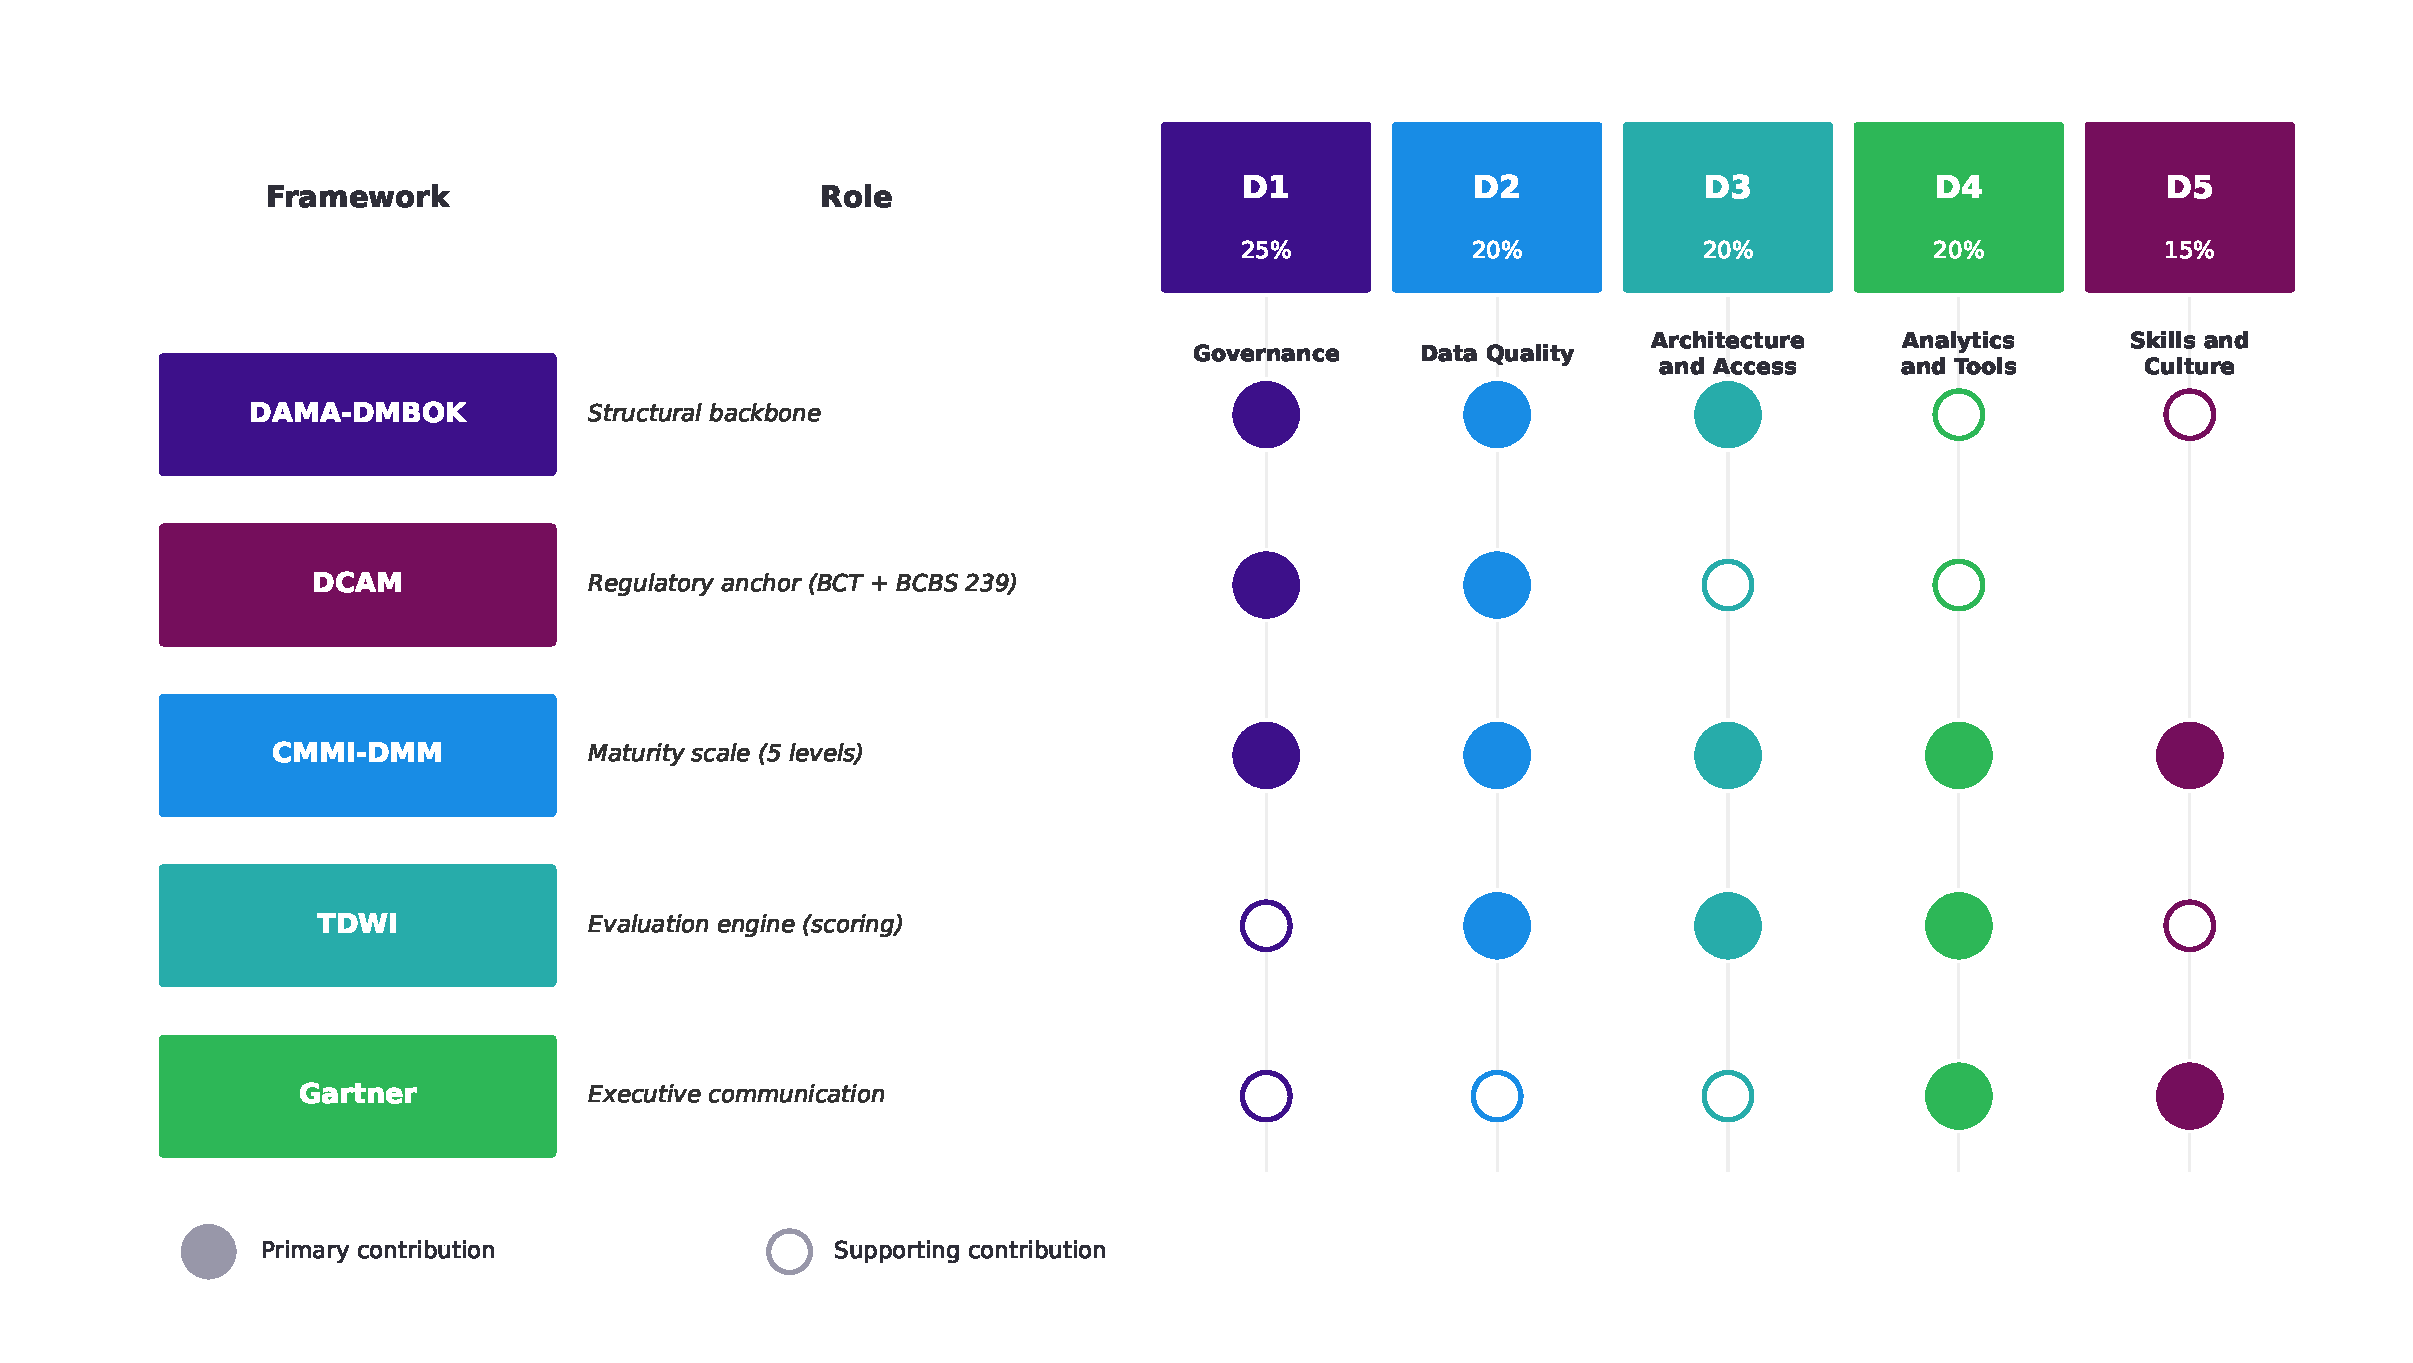
\includegraphics[width=0.9\textwidth]{images/hybrid-mapping.pdf}
\caption{Roles contributed by each benchmark to the hybrid framework. A filled circle marks a primary contribution and a hollow circle a supporting contribution.}
\label{fig:hybrid-mapping}
\end{figure}

\begin{table}[H]
\centering
\caption{Role, contribution, and exclusion for each selected framework} \label{tab:framework-roles}

{\footnotesize
\setlength{\tabcolsep}{4pt}
\begin{tabular}{|p{1.9cm}|p{2.3cm}|p{6.6cm}|p{3.7cm}|}
\hline
\textbf{Framework} & \textbf{Role} & \textbf{What was taken} & \textbf{What was excluded} \\
\hline
DAMA-DMBOK & Structural backbone & The 11 data management domains as a coverage reference; the taxonomy for the 5 dimensions and 12 sub-dimensions; definitions of data quality, lineage, and metadata scope & Scoring system (DAMA has none) \\
\hline
DCAM & Regulatory anchor & Banking-specific compliance logic (BCBS 239); the data ownership and accountability framework; the BCT Circulaire N\textdegree{}2025-08 alignment criteria & The full assessment process (too heavy for field use) \\
\hline
CMMI-DMM & Maturity scale & The 5-level maturity progression (Initial to Optimized); the principle that a practice is mature only when repeatable; level definitions and evidence-based scoring logic & The domain structure (replaced by DAMA's taxonomy) \\
\hline
TDWI & Evaluation engine & The structured questionnaire approach per dimension; per-indicator scoring rubrics for field consultants; the radar-chart output readable by non-technical management & The analytics-only focus (expanded to all 5 dimensions) \\
\hline
Gartner D\&A & Executive communication & The maturity labels (Unaware to Transformative); gap prioritization with effort and impact logic; the link between scores and business-value language & Proprietary tool dependency (replaced by an open model) \\
\hline
\end{tabular}
}

\end{table}

\subsection{Identified Research Gaps}

The review of existing frameworks reveals three gaps that motivate this project. First, no single framework is specific to the banking sector while also being aligned with the Tunisian regulatory environment defined by the BCT and BCBS 239. The one framework designed specifically for financial institutions covers the regulatory anchor well, but it is too heavy for a single field evaluation and does not natively encode the national circular. Meanwhile, the frameworks that are light enough to deploy are generic and blind to banking supervision. Second, the frameworks that are structurally rich are weak on operational scoring, while those that score well lack regulatory anchoring, so no framework offers both rigor and an auditable score out of the box. In particular, the most structurally complete reference provides no scoring system at all, and the frameworks that do score reliably were built for a narrower analytics scope. Neither can therefore produce a defensible maturity index across all five dimensions on its own. Third, none of the reviewed frameworks is delivered as a usable tool that bank management can operate directly. They exist as documents, proprietary services, or consulting engagements. None is delivered as an open instrument that a bank can run itself and that enforces the regulatory rules, the evidence requirement, and the maturity bands consistently.

Table~\ref{tab:framework-positioning} compresses these three gaps into a single positioning view: each row is a selected framework, each column a capability this project requires, and each cell records whether the framework provides it fully, partially, or not at all, as argued in the preceding subsections. The final row positions the present work against the same columns.

\begin{table}[H]
\centering
\caption{Positioning of the selected frameworks against the capability requirements of this work} \label{tab:framework-positioning}

{\footnotesize
\setlength{\tabcolsep}{4pt}
\begin{tabular}{|p{3.1cm}|p{2.1cm}|p{2.3cm}|p{2.1cm}|p{2.2cm}|p{2.0cm}|}
\hline
\textbf{Framework} & \textbf{Covers all five dimensions} & \textbf{Banking and regulatory alignment (BCT, BCBS 239)} & \textbf{Operational scoring method} & \textbf{Evidence requirement (anti-inflation)} & \textbf{Delivered as a usable tool} \\
\hline
DAMA-DMBOK & Yes & No & No & No & No \\
\hline
DCAM & Partial & Yes & Partial & Partial & No \\
\hline
CMMI-DMM & Partial & No & Yes & Partial & No \\
\hline
TDWI & No (analytics only) & No & Yes & No & No \\
\hline
Gartner D\&A & Partial & No & Partial & No & No (proprietary) \\
\hline
\textbf{DataPilot (this work)} & \textbf{Yes} & \textbf{Yes} & \textbf{Yes} & \textbf{Yes} & \textbf{Yes} \\
\hline
\end{tabular}
}

\end{table}

The empty columns map directly onto the research questions of Chapter 1. The absence of a framework that combines full coverage with banking and regulatory alignment means the sector has no instrument to measure its current state against the BCT and BCBS 239 expectations, which is what RQ1 sets out to do through the diagnostic. The gap between structural richness and operational, evidence-gated scoring defines the design problem of RQ2: a hybrid framework must be assembled that inherits the coverage of the first column, the regulatory anchor of the second, and the scoring mechanics of the third, and adds the evidence requirement that no source framework enforces. Finally, the uniformly empty tool column is the gap RQ3 addresses: without a directly operable instrument, even a well designed framework remains a document, and the assessment it describes cannot be run, repeated, or compared across institutions.

The project addresses these gaps by combining the frameworks into a hybrid model, equipping it with an auditable scoring methodology, and operationalizing it through an interactive tool. The hybrid model draws its structural taxonomy, regulatory anchor, maturity scale, evaluation mechanics, and executive communication layer from the five complementary frameworks. The scoring methodology adds an evidence requirement and a graded, renormalized index. The tool encodes both so that the assessment is reproducible across institutions. In doing so it closes the gap no existing framework closes on its own: a banking-specific, regulation-aligned, evidence-based, and directly operable data maturity assessment for the Tunisian context.

\subsection{Conclusion}

This chapter reviewed the banking and regulatory context, the concept of data maturity, and the five international frameworks that inform the design, and it identified the gaps the project addresses. The next chapter presents the methodology adopted to design and validate the artifacts.
